\documentclass[../main.tex]{subfiles}
\graphicspath{{\subfix{../Images/}}}
\begin{document}

%\section{YOLO} \label{yolo}
% Purpose and Context
The eighth generation of the \ac{YOLO} object detection framework developed by Ultralytics was selected to provide a high-performance, real-time vision baseline for this research. 
% \textcolor{red}{add something about semantic and information-rich data?}
This method of detection gained popularity for its ease of use and implementation for detecting and localizing objects within an image.
Once detected, an object is bounded by a rectangle that defines the minimum and maximum extremes of the pixel coordinates it occupies - known as the bounding box.
Its open-source models are pretrained on the COCO dataset, a large repository containing approximately 1.5 million labeled images, and are provided in various sizes and qualities, which can be deployed on a wide variety of edge computing hardware.
Additionally, transfer learning is simple to apply, allowing these models to be tailored for more specific use cases, such as maritime environments.

\begin{figure}
    \centering
    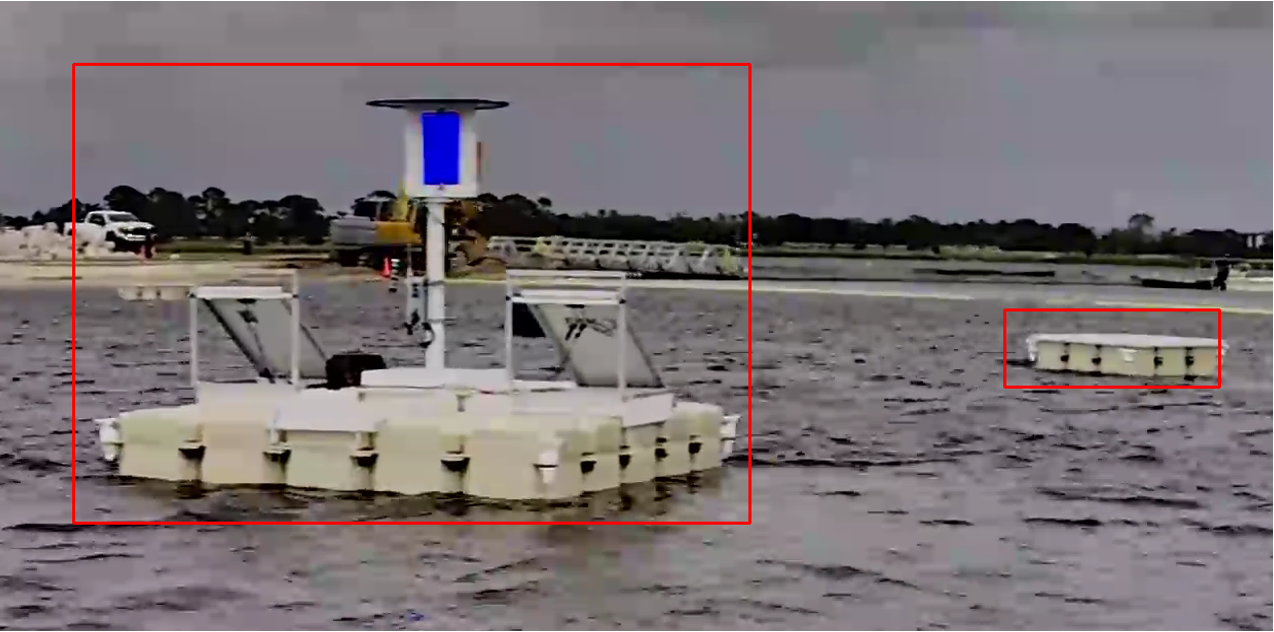
\includegraphics[width=0.5\linewidth]{Images/YOLO_ex1.png}
    \caption{Rectangular bounding boxes placed around maritime objects detected by a re-trained YOLO detection model.}
    \label{fig:YOLO_tower}
\end{figure}

The name YOLO refers to the one-shot convolutional neural network utilized to perform both detection and localization in a single pass of the network.
This architecture is what makes it fast, and for real-time object detection applications. 
Before the release of version 8 in 2023, the dual action of detection and localization required that the location and dimension of the bounding box also had to be encoded into the model.
Version 8 was the first to utilize dual-detection heads at the end of the CNN.
The first detection head identifies if and where an object is present within the image, and the second is used to determine the bounding box for the object.
This "anchor-free" architectural change not only makes localization of the detected objects more reliable, but also alleviates some of the intense transfer learning burden that was required for fine-tuning the pretrained models in earlier versions \cite{ultralytics}.

The widespread adoption of YOLOv8 and the fundamental architectural changes in this version make it the optimal choice to provide a baseline visual detection method.
% However, this mode of detection is not without its compromises, \textcolor{red}{as will be detailed in Section ____.}







% The YOLO Framework
% Describe the principle succinctly:

% YOLOv8 Architecture
% This section should flow from general framework to version-specific improvements:

% Image Resolution and Input Scaling
% Transition to operational detail and experimental consistency:

% Detection Scale and Spatial Sensitivity
% Discuss how feature maps relate to the detection limit:

% Model Constraints and Applicability
% Then note practical limitations and their relevance:

% Implications for Real-Time Fusion
% Conclude the section by connecting to your larger research goal:

% \textcolor{red}{To establish a performance baseline for real-time, vision-based object detection, this study employed the You Only Look Once (YOLO) framework, a single-stage convolutional neural network (CNN) architecture designed for end-to-end detection and classification. Unlike two-stage detectors that separately generate region proposals before classification, YOLO formulates detection as a direct regression problem, predicting bounding box coordinates and class probabilities simultaneously. This design allows all detections to occur in a single computational pass, providing the speed necessary for autonomous and embedded sensing applications. The visual detection results presented here serve as the reference modality for comparison with LiDAR-based detection methods and for evaluating computational performance in the subsequent late-fusion framework.}

% \textcolor{red}{
% The eighth-generation YOLOv8 model developed by Ultralytics was selected due to its stability, active development, and high inference efficiency on modern hardware. YOLOv8 integrates several architectural refinements that enhance accuracy and convergence speed relative to previous versions. The model employs an anchor-free detection strategy, eliminating the predefined bounding-box templates that characterized earlier YOLO iterations. Instead, YOLOv8 predicts the object center, width, and height directly, simplifying configuration and improving adaptability to objects of varying aspect ratios and scales. A decoupled detection head separates the regression and classification branches of the network, allowing independent optimization of spatial and semantic components during training. The backbone of the network uses C2f (Cross-Stage Partial Fusion) modules, which improve feature reuse and gradient flow while reducing overall computation. These modifications collectively contribute to higher accuracy and reduced latency, both of which are critical for on-board real-time inference
% The model employs modern loss functions to enhance bounding-box precision. The Complete-IoU (CIoU) loss function refines localization by incorporating geometric distance and aspect ratio penalties, while the Distribution-Focal Loss (DFL) improves boundary regression stability. Together, these losses improve the correspondence between predicted and ground-truth boxes and facilitate more consistent convergence during training. The network was implemented in PyTorch using the native Ultralytics framework, which provides integrated preprocessing, data augmentation, and export utilities. This implementation enables consistent deployment across GPU-based and embedded computing platforms without manual configuration
% }
% \textcolor{red}{
% All input frames were processed at a resolution of 640 × 640 pixels, which corresponds to YOLOv8’s default operational size and the native output of the experimental imaging system. Maintaining this native resolution avoided unnecessary interpolation and ensured a one-to-one correspondence between camera pixels and network input. YOLOv8 performs detection at three spatial scales, corresponding to feature-map strides of 8, 16, and 32 pixels relative to the input. These scales allow simultaneous sensitivity to small, medium, and large objects within a single inference pass. For a 640 × 640 input image, these feature maps have effective dimensions of 80 × 80, 40 × 40, and 20 × 20 cells, respectively. Each cell in the smallest-stride feature map represents an 8 × 8 pixel region of the input image.}
% \textcolor{red}{
% Because of this multi-scale design, the network’s minimum detectable object size is bounded by the stride of the smallest feature map. Objects must occupy multiple adjacent cells to generate distinct activations; those confined to a single cell are typically lost through downsampling or non-maximal suppression. Empirical evaluation and prior literature indicate that YOLOv8 reliably detects objects approximately 16–32 pixels in width or height—roughly 0.5–1 percent of the frame area for a 640 × 640 input. Objects smaller than this threshold generally produce low-confidence or unstable detections.}
% \textcolor{red}{
% This limitation arises from several interrelated factors. First, downsampling loss in convolutional and pooling layers reduces high-frequency detail, causing very small features to disappear from deeper network layers. Second, the receptive field of later layers covers large portions of the input image, diminishing the spatial specificity required for fine-scale detections. Third, training bias inherent to datasets such as COCO and VOC, which contain relatively large annotated objects, restricts the network’s learned sensitivity to sub-pixel features. These factors collectively define the lower bound of object detectability in standard YOLOv8 configurations.}
% \textcolor{red}{
% The 640 × 640 camera used in this study matches the network’s native input dimension, permitting direct inference without rescaling and ensuring consistent timing measurements for real-time operation. This configuration provides an accurate representation of YOLOv8’s performance under embedded deployment conditions and serves as a visual-only detection baseline against which LiDAR-based methods and fused detection results are compared in later sections. The analysis presented here therefore defines the temporal and computational characteristics of the visual detection pipeline that underpin the late-fusion approach adopted in this research.
% }

%%%%%%%%%%%%%%%%%%%%%%%%%%%%%%%%%%%%%%%%%%%%%%%%%%%%%%%%%%%%%%%%%%%%
%%%%%%%%%%%%%%%%%%%%%%%%%%%%%%%%%%%%%%%%%%%%%%%%%%%%%%%%%%%%%%%%%%%%

\end{document}
